%==============================================================
% Seminário — Processamento Digital de Imagens (UFAM)
% Artigo: Improved image segmentation method based on
%         morphological reconstruction (Wu et al., 2017)
%         Multimed Tools Appl 76:19781-19793 — DOI 10.1007/s11042-015-3192-2
%==============================================================
\documentclass[aspectratio=169,12pt]{beamer}

\usepackage[T1]{fontenc}
\usepackage[utf8]{inputenc}
\usepackage[brazil]{babel}
\usepackage{amsmath,amssymb,amsfonts}
\usepackage{mathtools}
\usepackage{booktabs}
\usepackage{array}
\usepackage{xcolor}
\usepackage{graphicx}
\usepackage{tikz}
\usepackage{pgfplots}
\usetikzlibrary{arrows.meta, positioning, shapes.geometric}
\pgfplotsset{compat=1.18}

%==============================================================
% TEMA E CORES UFAM
%==============================================================
\usetheme{Madrid}
\usecolortheme{default}

\definecolor{ufamblue}{RGB}{0,51,102}
\definecolor{ufamlightblue}{RGB}{0,102,170}
\definecolor{ufamgold}{RGB}{204,153,0}
\definecolor{ufamgreen}{RGB}{0,102,51}
\definecolor{boxbg}{RGB}{240,248,255}

\setbeamercolor{palette primary}{bg=ufamblue, fg=white}
\setbeamercolor{palette secondary}{bg=ufamlightblue, fg=white}
\setbeamercolor{palette tertiary}{bg=ufamgold, fg=black}
\setbeamercolor{palette quaternary}{bg=ufamblue, fg=white}
\setbeamercolor{structure}{fg=ufamblue}
\setbeamercolor{section in toc}{fg=ufamblue}
\setbeamercolor{frametitle}{bg=ufamblue, fg=white}
\setbeamercolor{title}{bg=ufamblue, fg=white}
\setbeamercolor{block title}{bg=ufamlightblue, fg=white}
\setbeamercolor{block body}{bg=boxbg, fg=black}
\setbeamercolor{block title alerted}{bg=ufamgold, fg=black}
\setbeamercolor{block body alerted}{bg=yellow!10, fg=black}
\setbeamercolor{block title example}{bg=ufamgreen, fg=white}
\setbeamercolor{block body example}{bg=green!5, fg=black}

\setbeamerfont{frametitle}{size=\large, series=\bfseries}
\setbeamerfont{title}{size=\Large, series=\bfseries}
\setbeamertemplate{navigation symbols}{}
\setbeamertemplate{caption}[numbered]

\setbeamertemplate{footline}{
  \leavevmode
  \hbox{
    \begin{beamercolorbox}[wd=.33\paperwidth,ht=2.5ex,dp=1.5ex,center]{palette primary}
      \usebeamerfont{author in head/foot}\insertshortauthor
    \end{beamercolorbox}
    \begin{beamercolorbox}[wd=.34\paperwidth,ht=2.5ex,dp=1.5ex,center]{palette secondary}
      \usebeamerfont{title in head/foot}\insertshorttitle
    \end{beamercolorbox}
    \begin{beamercolorbox}[wd=.33\paperwidth,ht=2.5ex,dp=1.5ex,center]{palette primary}
      \usebeamerfont{date in head/foot}\insertframenumber\,/\,\inserttotalframenumber
    \end{beamercolorbox}
  }
}

%==============================================================
% METADADOS
%==============================================================
\title[Segmentação por Reconstrução Morfológica]{Improved Image Segmentation Method\\Based on Morphological Reconstruction}
\subtitle{Seminário --- Processamento Digital de Imagens}
\author[Matheus Serrão Uchôa]{Matheus Serrão Uchôa}
\institute[UFAM]{\textbf{Universidade Federal do Amazonas} --- Instituto de Computação}
\date{Manaus, \today}

% Referência do artigo
\newcommand{\artigo}{\textit{Wu, Peng, Ruan \& Hu.} Multimed Tools Appl \textbf{76}:19781--19793 (2017)}

%==============================================================
\begin{document}
%==============================================================

%--------------------------------------------------------------
% CAPA
%--------------------------------------------------------------
\begin{frame}[plain]
  \begin{tikzpicture}[remember picture, overlay]
    \fill[ufamblue] (current page.north west) rectangle
      ([yshift=-2.2cm]current page.north east);
    \fill[ufamgold] ([yshift=-2.2cm]current page.north west) rectangle
      ([yshift=-2.5cm]current page.north east);
    \fill[ufamblue!20] (current page.south west) rectangle
      ([yshift=1.2cm]current page.south east);
    \node[anchor=south east] at ([xshift=-0.5cm,yshift=0.3cm]current page.south east)
      {
\includegraphics[height=1.3cm]{figs/ufam_logo.png}};
  \end{tikzpicture}
  \vspace{0.5cm}
  \titlepage
  \begin{center}\small
    Artigo original: \artigo\\
    DOI: 10.1007/s11042-015-3192-2
  \end{center}
\end{frame}

%--------------------------------------------------------------
% SUMÁRIO
%--------------------------------------------------------------
\begin{frame}{Sumário}
  \tableofcontents[hideallsubsections]
\end{frame}

%==============================================================
\section{Contexto e Motivação}
%==============================================================
\begin{frame}{Contexto: segmentação de imagens}
  \begin{block}{O problema}
    A \textbf{segmentação} é o elo entre processamento e análise de imagens ---
    extrai características significativas (bordas, regiões) para reconhecimento
    e interpretação. É um problema central em visão computacional.
  \end{block}
  \begin{columns}[T]
    \begin{column}{0.5\textwidth}
      \textbf{Abordagens clássicas:}
      \begin{itemize}
        \item por \alert{limiar} (threshold)
        \item por \alert{região} (area)
        \item por \alert{borda} (edge)
      \end{itemize}
    \end{column}
    \begin{column}{0.5\textwidth}
      \textbf{Aplicação-alvo do artigo:}
      \begin{itemize}
        \item imagens de \alert{espuma de flotação} (\textit{froth}) na mineração
        \item bolhas de \alert{tamanhos muito variados} na mesma imagem
      \end{itemize}
    \end{column}
  \end{columns}
  \vspace{0.3cm}
  \begin{exampleblock}{Watershed (divisor de águas)}
    Método de segmentação por região baseado em morfologia matemática, muito
    usado; encontra bordas por conjuntos fechados conexos.
  \end{exampleblock}
\end{frame}

\begin{frame}{A motivação: limitação do watershed tradicional}
  \begin{columns}[T]
    \begin{column}{0.52\textwidth}
      \begin{alertblock}{Limiar único não funciona}
        Um \textbf{único limiar} não consegue, ao mesmo tempo:
        \begin{itemize}
          \item eliminar ruído dentro de bolhas \alert{grandes}; e
          \item realçar as bordas de bolhas \alert{pequenas}.
        \end{itemize}
      \end{alertblock}
      \begin{itemize}
        \item Limiar \textbf{baixo} $\Rightarrow$ \alert{super-segmentação}
              (over-segmentation)
        \item Limiar \textbf{alto} $\Rightarrow$ \alert{sub-segmentação}
              (under-segmentation)
      \end{itemize}
    \end{column}
    \begin{column}{0.48\textwidth}
      \begin{figure}
        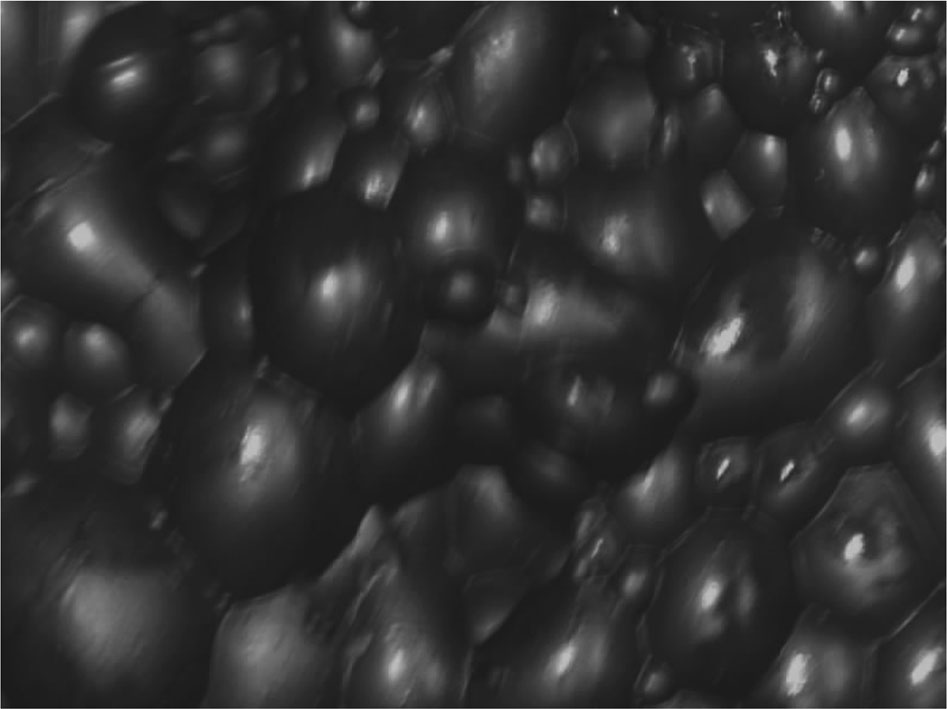
\includegraphics[width=\textwidth]{figs/froth_original.png}
        \caption{Imagem de espuma (\textit{froth}) com bolhas de diversos tamanhos.}
      \end{figure}
    \end{column}
  \end{columns}
\end{frame}

\begin{frame}{Objetivo e contribuição}
  \begin{block}{Objetivo}
    Propor um método de segmentação baseado em \textbf{reconstrução morfológica}
    que trate corretamente objetos de \textbf{tamanhos diferentes}, reduzindo a
    super-segmentação do watershed.
  \end{block}
  \begin{block}{Ideia central}
    Usar \textbf{limiares diferentes} para diferentes faixas de tamanho de objeto,
    marcando e \textbf{remodelando} as bacias de captação (\textit{catchment
    basins}) por operações morfológicas (erosão/dilatação) antes de aplicar o
    watershed sobre os marcadores.
  \end{block}
\end{frame}

%==============================================================
\section{Fundamentos: Morfologia Matemática}
%==============================================================
\begin{frame}{Operações morfológicas binárias}
  Sejam $A, B \subseteq \mathbb{Z}^2$ ($B$ = elemento estruturante).
  \vspace{0.2cm}
  \begin{columns}[T]
    \begin{column}{0.5\textwidth}
      \begin{block}{Dilatação $A \oplus B$}
        \[ A \oplus B = \{\, x : \hat{B}_x \cap A \neq \varnothing \,\} \]
        Expande objetos; \alert{une} bacias vizinhas.
      \end{block}
      \begin{block}{Erosão $A \ominus B$}
        \[ A \ominus B = \{\, x : B_x \subseteq A \,\} \]
        Encolhe objetos; \alert{remove} interior das bacias.
      \end{block}
    \end{column}
    \begin{column}{0.5\textwidth}
      \begin{block}{Abertura $A \circ B$}
        \[ A \circ B = (A \ominus B) \oplus B \]
        Erosão seguida de dilatação (suaviza contornos).
      \end{block}
      \begin{block}{Fechamento $A \bullet B$}
        \[ A \bullet B = (A \oplus B) \ominus B \]
        Dilatação seguida de erosão (preenche buracos).
      \end{block}
    \end{column}
  \end{columns}
  \vspace{0.15cm}
  \footnotesize $\hat{B}$: reflexão de $B$; \; $B_x$: translação de $B$ por $x$.
\end{frame}

\begin{frame}{Watershed e transformação H-mínima}
  \begin{block}{Watershed (L. Vincent): duas etapas}
    \textbf{Ordenação} (pixels do menor ao maior nível de cinza) $\;\to\;$
    \textbf{inundação} (\textit{submerging}) a partir dos mínimos locais.
  \end{block}
  \begin{exampleblock}{Marcação das bacias --- transformação H-mínima}
    \[ H_{\min}(f) = R_\epsilon^{\,f}(f + h) \tag{11} \]
    \small $f$: imagem original; \; $h$: profundidade da bacia; \;
    $R_\epsilon$: reconstrução por erosão. Cada mínimo local vira uma
    \textbf{bacia de captação} (semente do watershed).
  \end{exampleblock}
  \begin{alertblock}{O papel da morfologia}
    \textbf{Erosão} reduz sub-segmentação (remove interior da bacia); \;
    \textbf{dilatação} reduz super-segmentação (funde bacias próximas).
  \end{alertblock}
\end{frame}

\begin{frame}{O sintoma: super-segmentação}
  \begin{columns}[c]
    \begin{column}{0.5\textwidth}
      \centering
      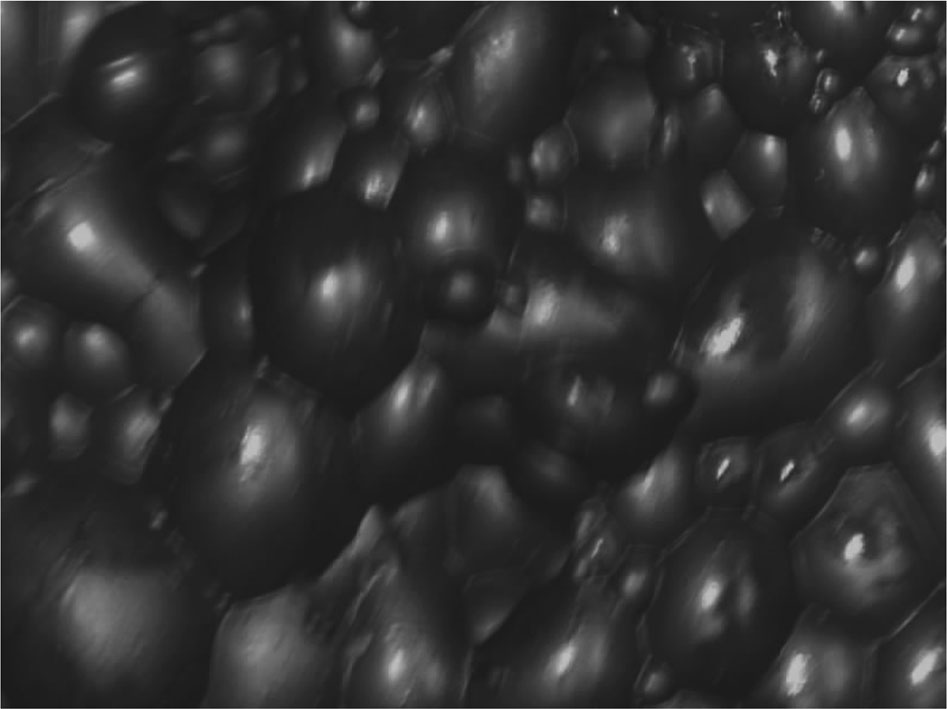
\includegraphics[width=\textwidth]{figs/froth_original.png}\\
      \small (a) Imagem original
    \end{column}
    \begin{column}{0.5\textwidth}
      \centering
      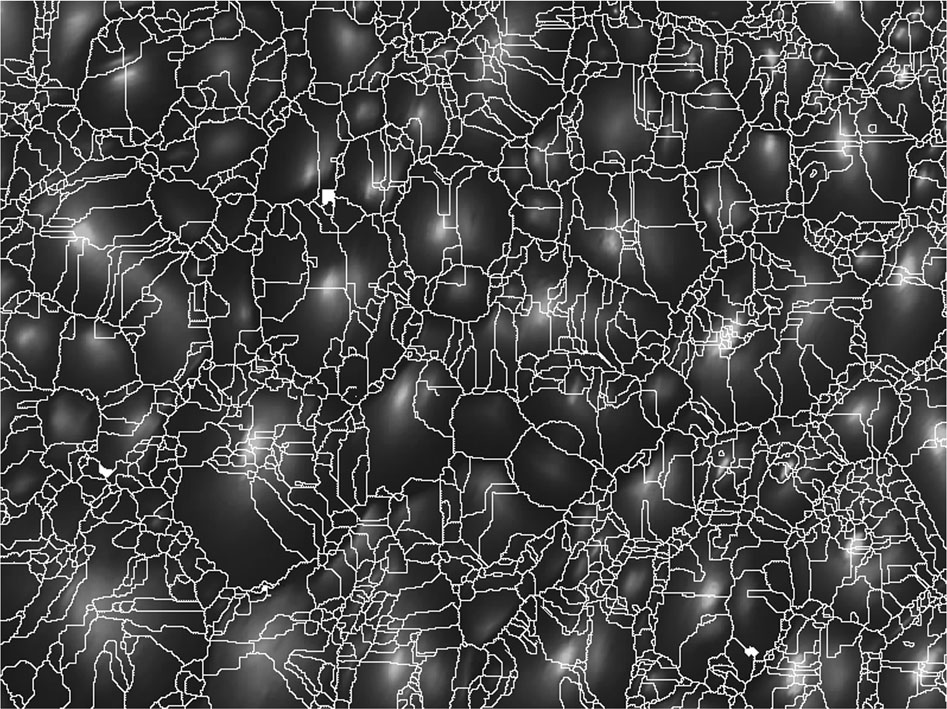
\includegraphics[width=\textwidth]{figs/froth_oversegmentation.png}\\
      \small (b) Watershed \alert{puro} $\Rightarrow$ super-segmentação
    \end{column}
  \end{columns}
  \vspace{0.3cm}
  \centering
  Aplicar watershed diretamente gera \alert{centenas de regiões espúrias}
  --- bordas onde não há bolhas.
\end{frame}

%==============================================================
\section{Método Proposto}
%==============================================================
\begin{frame}{Método proposto --- visão geral (6 passos)}
  \centering
  \scriptsize
  \begin{tikzpicture}[
      node distance=0.35cm and 0.5cm,
      box/.style={rectangle, rounded corners, draw=ufamblue, very thick,
        fill=boxbg, text width=2.5cm, align=center, minimum height=1.1cm},
      arr/.style={-{Stealth[length=3mm]}, ufamgold, very thick}]
    \node[box] (s1) {\textbf{1.} Transf.\ H-mínima (bacias iniciais)};
    \node[box, right=of s1] (s2) {\textbf{2.} Verificação por \'area (classificar)};
    \node[box, right=of s2] (s3) {\textbf{3.} Remodelagem morfol\'ogica (dilata/erode)};
    \node[box, below=of s3] (s4) {\textbf{4.} Inversão $g=255-f$};
    \node[box, left=of s4] (s5) {\textbf{5.} Watershed sobre marcadores};
    \node[box, left=of s5] (s6) {\textbf{6.} Reinversão (resultado)};
    \draw[arr] (s1) -- (s2);
    \draw[arr] (s2) -- (s3);
    \draw[arr] (s3) -- (s4);
    \draw[arr] (s4) -- (s5);
    \draw[arr] (s5) -- (s6);
  \end{tikzpicture}
  \vspace{0.3cm}
  \begin{block}{Chave do método}
    Buscar as bacias corretas com \textbf{limiares $H$ distintos por faixa de
    tamanho}, e usar os marcadores remodelados como \textbf{sementes} do watershed.
  \end{block}
\end{frame}

\begin{frame}{Passos 1--3: marcar, classificar e remodelar}
  \begin{columns}[T]
    \begin{column}{0.55\textwidth}
      \textbf{Passo 1 --- Transformação H-mínima}\\
      Com limiar de profundidade adequado, extrai as bacias iniciais
      (grandes, médias e pequenas).
      \vspace{0.25cm}

      \textbf{Passo 2 --- Verificação}\\
      Classificar e coletar bacias pela \alert{medida de área}; garantir que
      cada uma esteja na faixa correta.
      \vspace{0.25cm}

      \textbf{Passo 3 --- Remodelagem morfológica}\\
      Dilatação proporcional à área (\alert{quanto maior a bacia, maior a
      dilatação}); sobrepõe tudo em uma imagem e aplica erosão.
    \end{column}
    \begin{column}{0.45\textwidth}
      \begin{figure}
        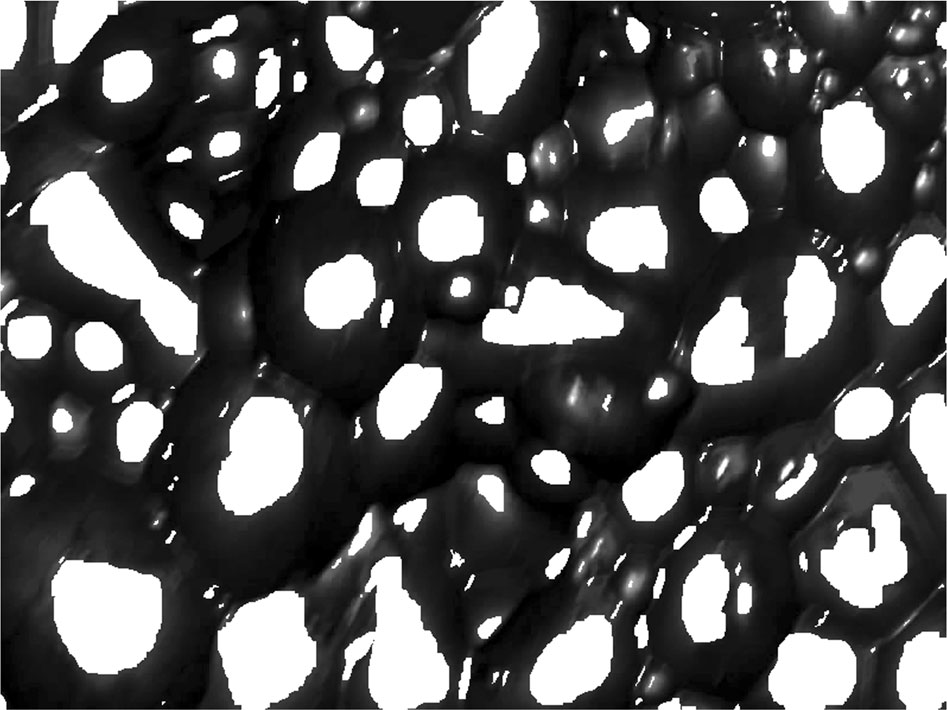
\includegraphics[width=\textwidth]{figs/froth_markers.png}
        \caption{Bacias remodeladas (marcadores) $\approx$ elipses, coerentes
        com as bolhas reais.}
      \end{figure}
    \end{column}
  \end{columns}
\end{frame}

\begin{frame}{Passos 4--6: inverter, segmentar, reduzir}
  \begin{block}{Passo 4 --- Inversão}
    Inverte o nível de cinza para transformar \textbf{picos em vales}:
    \[ g(x,y) = 255 - f(x,y) \]
    (assim os marcadores tornam-se os mínimos que a inundação preenche).
  \end{block}
  \begin{block}{Passo 5 --- Segmentação de bordas}
    Aplica o \textbf{watershed} usando a imagem invertida (marcadores) como
    \alert{área de sementes}.
  \end{block}
  \begin{block}{Passo 6 --- Redução}
    Inverte novamente a imagem. O resultado fica \textbf{em correspondência
    direta} com as bacias obtidas --- cada bolha, grande ou pequena.
  \end{block}
\end{frame}

%==============================================================
\section{Experimentos e Resultados}
%==============================================================
\begin{frame}{Parâmetros experimentais (Tabela 1)}
  \centering
  \begin{block}{Quatro faixas de bacia de captação}
    \renewcommand{\arraystretch}{1.3}
    \begin{tabular}{lcccc}
      \toprule
      & \textbf{Little} & \textbf{Small} & \textbf{Middle} & \textbf{Large} \\
      \midrule
      Faixa de área (px)          & $[2,12]$ & $[12,120]$ & $[120,1200]$ & $[1200,40000]$ \\
      Limiar $H$-mínimo           & 20 & 30 & 50 & 80 \\
      Coef.\ de dilatação         & 0 & 2 & 4 & 8 \\
      \bottomrule
    \end{tabular}
  \end{block}
  \vspace{0.3cm}
  \begin{itemize}
    \item Cada faixa de tamanho tem seu \alert{próprio limiar} e sua \alert{própria
          dilatação}.
    \item Bacias maiores recebem dilatação mais intensa --- daí a remodelagem
          "por tamanho".
  \end{itemize}
\end{frame}

\begin{frame}{Resultado da segmentação proposta}
  \begin{columns}[c]
    \begin{column}{0.5\textwidth}
      \centering
      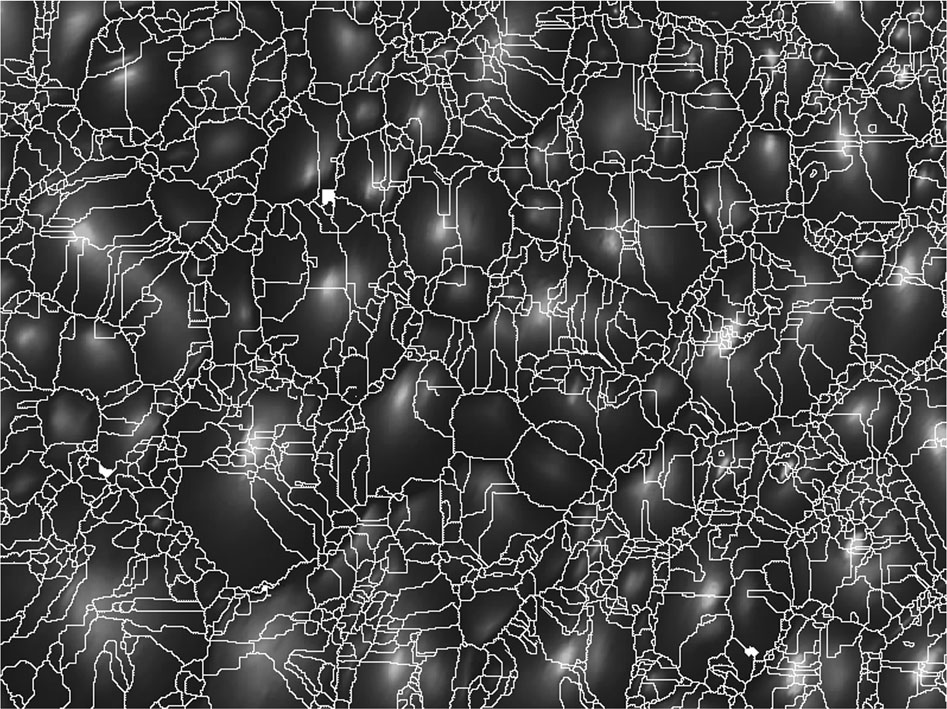
\includegraphics[width=\textwidth]{figs/froth_oversegmentation.png}\\
      \small Watershed puro (super-segmentado)
    \end{column}
    \begin{column}{0.5\textwidth}
      \centering
      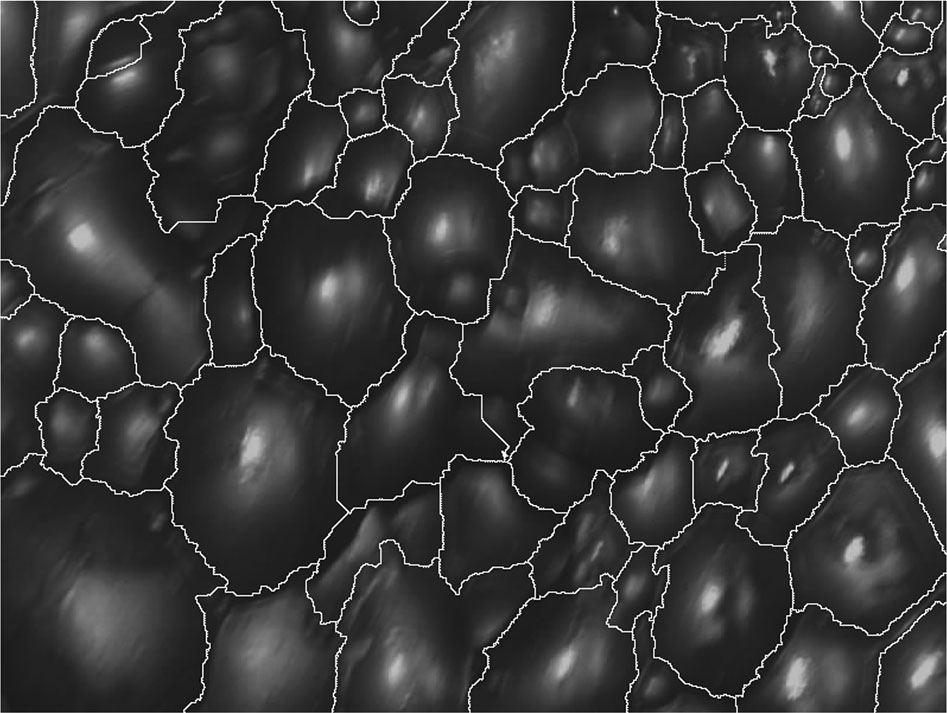
\includegraphics[width=\textwidth]{figs/froth_result.png}\\
      \small \textbf{Método proposto} (reconstrução morfológica)
    \end{column}
  \end{columns}
  \vspace{0.25cm}
  \centering
  As regiões passam a corresponder \alert{uma a uma} às bolhas reais ---
  grandes e pequenas.
\end{frame}

\begin{frame}{Comparação de acurácia (Fig.\ 9)}
  \centering
  \begin{tikzpicture}
    \begin{axis}[
        width=0.82\textwidth, height=0.62\textheight,
        xlabel={Sequência de imagens de espuma},
        ylabel={\'Areas segmentadas corretamente (\%)},
        xmin=0, xmax=25, ymin=40, ymax=100,
        legend pos=south west, legend style={font=\scriptsize},
        grid=both, grid style={gray!20},
        tick label style={font=\footnotesize},
        label style={font=\footnotesize}]
      % Método proposto (>80%)
      \addplot[ufamgreen, very thick, mark=*, mark size=1.2pt] coordinates {
        (1,84)(3,86)(5,83)(7,88)(9,85)(11,87)(13,82)(15,86)(17,89)(19,84)(21,87)(23,85)(25,88)};
      \addlegendentry{Método proposto}
      % Comprehensive watershed (~65-75%)
      \addplot[ufamlightblue, very thick, mark=square*, mark size=1.2pt] coordinates {
        (1,70)(3,68)(5,72)(7,66)(9,71)(11,69)(13,73)(15,67)(17,70)(19,72)(21,68)(23,71)(25,69)};
      \addlegendentry{Watershed abrangente}
      % Gradient transformation (~50-62%)
      \addplot[ufamgold!80!black, very thick, mark=triangle*, mark size=1.4pt] coordinates {
        (1,56)(3,54)(5,60)(7,52)(9,58)(11,55)(13,61)(15,53)(17,57)(19,59)(21,54)(23,58)(25,56)};
      \addlegendentry{Transf.\ por gradiente}
    \end{axis}
  \end{tikzpicture}\\
  \footnotesize Tendência reproduzida a partir da Fig.\ 9 do artigo: o método
  proposto mantém acurácia \alert{$>80\%$} com alta robustez.
\end{frame}

\begin{frame}{Análise dos resultados}
  \begin{enumerate}
    \item \textbf{Limiar controla o regime:} $H$ baixo $\Rightarrow$ super-segmentação;
      $H$ alto $\Rightarrow$ sub-segmentação.
    \item \textbf{Tamanho $\leftrightarrow$ limiar:} após dilatação + erosão as
      bacias ficam elípticas; bacias próximas se fundem, ficando coerentes com as
      bolhas.
    \item \textbf{Limitação:} ainda restam algumas regiões super/sub-segmentadas;
      uma classificação mais fina das bacias melhoraria o resultado.
    \item \textbf{Ganho principal:} limiares distintos em diferentes espaços de
      cinza resolvem o descasamento de bolhas de tamanhos diferentes ---
      acurácia \alert{$>80\%$}, superior aos métodos tradicionais.
  \end{enumerate}
\end{frame}

%==============================================================
\section{Conclusão}
%==============================================================
\begin{frame}{Conclusão}
  \begin{block}{Contribuição}
    Algoritmo que melhora a segmentação por \textbf{reconstrução morfológica},
    adequado a imagens de espuma com bolhas \textbf{grandes e pequenas}.
  \end{block}
  \begin{itemize}
    \item Marcadores obtidos por \textbf{transformação H-mínima} e separados por
      \textbf{tamanho}, com transformação morfológica correspondente.
    \item Watershed aplicado sobre os \textbf{marcadores remodelados} como sementes.
    \item Todas as bacias --- grandes ou pequenas --- ficam em correspondência
      \textbf{um a um} com as bolhas reais.
  \end{itemize}
  \begin{exampleblock}{Mensagem central}
    Trocar \emph{um limiar global} por \emph{marcadores morfológicos por faixa de
    tamanho} controla a super-segmentação do watershed em cenas com objetos de
    escalas muito diferentes.
  \end{exampleblock}
\end{frame}

\begin{frame}[plain]
  \begin{tikzpicture}[remember picture, overlay]
    \fill[ufamblue] (current page.center) ++(-\paperwidth/2,-1.6cm)
      rectangle ++(\paperwidth,3.2cm);
  \end{tikzpicture}
  \centering
  \vspace{1.2cm}
  {\color{white}\Large\bfseries Obrigado!}\\[0.3cm]
  {\color{white} Perguntas?}\\[1.2cm]
  \small
  \artigo\\
  DOI: 10.1007/s11042-015-3192-2
\end{frame}

\end{document}
